\chapter{Using LaTeX to make documents that meet NREL's requirements}

\section{What is LaTeX?}
LaTeX is a mark-up language that describes how a document should be prepared. Three things are needed to make a LaTeX document:
\begin{enumerate}
\item A source document, usually with extension \emph{.tex}
\item Some packages and classes that help turn what's in the source document into something helpful
\item A compiler, also referred to as a working LaTeX installation.
\end{enumerate}

At first glance the source document looks like a programming language, and that's because it is: LaTeX is not WYSIWYG, like many of the document preparation tools in common use today. A good analogy is html.

The wikibook at \href{http://en.wikibooks.org/wiki/LaTeX}{http://en.wikibooks.org/wiki/LaTeX} is an excellent resource. There are also several internet forums such as \href{tex.stackexchange.com}{tex.stackexchange.com} that may be useful.

\section{General Process}
An outline of the process for producing NREL documents using LaTeX{} is given in Table \ref{Tab:NRELprocess}. Please note that this process is subject to revision without warning.

\begin{table}[!h]
\centering
\caption{NREL's process for producing and reviewing LaTeX{} files}
\label{Tab:NRELprocess}
\begin{tabular*}{\textwidth}{llp{0.5\textwidth}r}
\toprule
Phase & Lead & Steps & More Information \\
\midrule
Draft & Author & 1. Prepare document in LaTeX using the \emph{nrel.cls} class file & Section \ref{sec:nrelcls} \\
 & & 2. Prepare PDF & Section \ref{sec:PDFprep} \\
 & & 3. Convert the tex document to a word processing format (\emph{.rtf, .doc, .docx}) using a tool such as  \texttt{latex2rtf} or \texttt{pandoc} & Chapter \ref{sec:latextodoc}\\
 & & 5. Archive all files, including:
\begin{itemize}  
 \item LaTeX source files
 \item Images
 \item Final PDF 
 \end{itemize} & \\
Review & Communications & Review the structure of the PDF & \\
 & & Edit the supplied \emph{.doc} or \emph{.docx} file using track changes & \\
Revision & Author & Implements required changes in the LaTeX files. & \\
&  & Create the final, tagged and structured PDF \\
Publish & Publications & Combine the PDF with the appropriate cover sheet(s) & \\
\bottomrule
\end{tabular*}
\end{table}

\section{The NREL LaTeX style file}\label{sec:nrelcls}
A LaTeX class called \emph{nrel.cls} has been written that implements the NREL formatting requirements in LaTeX.

\subsection{Getting nrel.cls}
The current version of \emph{nrel.cls} can be downloaded from \href{https://github.com/NREL/latex_editing}{https://github.com/NREL/latex\_editing}. This is a public repository.

\subsection{Installing nrel.cls}
Place \emph{nrel.cls} and \emph{nrel.bst} in the same directory as the LaTeX files you are trying to compile. This will make the files available to that project, only. This approach can be used on a desktop computer, or on a network drive, or for online collaborative tools such as \href{www.writelatex.com}{www.writelatex.com} or \href{www.sharelatex.com}{www.sharelatex.com}. Advanced LaTeX users may wish to copy these files to their local tree.

\subsection{Using nrel.cls}
To use the class file, insert the following text in the preamble, before \verb+\begin{document}+:

\begin{verbatim}
\newif\iflatextortf

\iflatextortf
 % tell latex2tortf if this is an article or report
 \documentclass[10pt,letterpaper]{report}
 % File NRELLatex2rtf.tex

% set margins
\usepackage[margin=1 in,letterpaper]{geometry}

% use citations
\usepackage[sort]{natbib}

% change the heading of the bibliography
\renewcommand{\bibsection}{\section{References}}

% redefine \pdftooltip so that it behaves differently with and without latextortf
\newcommand{\pdftooltip}[3][]{#2}

%redefine the checkmark
\newcommand{\checkmark}{y\relax}

% redefine booktabs commands
\newcommand{\toprule}{\hline}
\newcommand{\midrule}{\hline}
\newcommand{\bottomrule}{\hline}

% redefine \href
\newcommand{\href}[2]{#1~ (\url{#2})}

% redefine \subfloat to match the \subfigure environment
\usepackage{subfigure}
\makeatletter
\newcommand{\subfloat}[2][]{\subfigure{\textit{Subcaption: \protect{#1}}}{#2}}
%\newcommand{\subfloat}[3][]{\subfigure{#1}{#2}{#3}}
% note that we can only have one '\label' in a figure environment
\makeatother

\newcommand{\subref}[1][]{\ref{#1}}

% redefine \todo so that it gives something useful
\newcommand{\todo}[2][]{\textbf{To Do:}~#2}

% deal with index entries:
\newcommand{\index}[1]{}
\else
 \documentclass[draft,report]{nrel} 
\fi
\end{verbatim}

This tells LaTeX to use the correct class file, and defines a set of commands that will be used by \emph{latextortf} to properly convert the latex to a rich text document for reviewing (see Chapter \ref{sec:latextortf}).

\subsection{Options in nrel.cls}\label{sec:nrel.cls.options}
The line

\begin{verbatim}
\documentclass[draft,report]{nrel}
\end{verbatim}

\noindent specifies the options (inside the square brackets) that will be passed to the \emph{nrel} class. The options include:
\begin{description}
\item[book]{compile the document using the LaTeX \emph{book} class. This is intended for longer documents and allows the use of chapters.}
\item[report]{compile the document using the LaTeX \emph{report} class. This is intended for longer documents and allows the use of chapters.}
\item[article]{compile the document using the LaTeX \emph{article} class. This is intended for shorter documents such as journal articles. This class does not support the use of chapters.}
\item[memoir]{compile the document using the LaTeX \emph{memoir} class. This option is not recommended because of the challenge with later converting to RTF format for communications review.}
\item[draft]{add a `draft' watermark to all pages and colours all links in blue.}
\item[10pt, 12pt]{set the font size accordingly. The default is 12 point.}
\item[letterpaper, a4paper]{set the paper size. the default is letter paper.}
\end{description}

\subsection{Classes and packages in nrel.cls}
\emph{nrel.cls} calls a variety of other packages. Packages are codes that modify the appearance or behaviour of LaTeX to achieve something. Table \ref{Tab:Packages} lists the packages that are explicitly called by \emph{nrel.cls} in the order they are called in. These packages often call other packages, so this is not an exhaustive list.

\begin{table}[!h]
\centering
\caption[Packages supported by the nrel.cls class]{Packages supported by nrel.cls. Unless otherwise stated, packages are not supported by latex2rtf.}
\label{Tab:Packages}
\begin{tabular*}{\textwidth}{p{0.125\textwidth}p{0.1\textwidth}p{0.4\textwidth}p{0.25\textwidth}}
\toprule
Packages & options & functionality & \texttt{latex2rtf} support \\
\midrule
nag & & checks that packages are up to date and looks for bad habits in LaTeX code. & \\
geometry & & sets page size and margins & \checkmark\\
mathptmx& & changes fonts & \\
helvet& & changes fonts & \\
courier& & changes fonts & \\
amsfonts, amssymb & & supplies the AMS fonts, which are useful for mathematics & \\
booktabs & & & \\
graphicx & &graphics handling, including \emph{.eps} figures & \checkmark\\
natbib & sort &handles citations and allows the \verb+\cite+, \verb+\citep+ and \verb+\citet+ citation commands (see Section \ref{Sec:Bib}). & \checkmark\\
fontenc & T1 & &\\
xcolor & & &\\
babel & english & &\\
subfigure & & provides the \texttt{subfigure} environment to produce sub figures & \checkmark \\
hyphenat & & &\\
setspace & & &\\
parskip & & &\\
toclof & subfigure & & \\
toclifbind & nottoc, notlot, notlof & &\\
todonotes & & inline and margin to-do notes & \checkmark (`to do' is prefaced with \textbf{To Do:} in the output)\\
listings & & & \\
caption & & &\\
pdfcomment & & tool-tips. Also calls the package \texttt{hyper ref} & \checkmark (the tool tip is suppressed) \\
accessibility & tagged & generates the document structure and tagging & \\
\bottomrule
\end{tabular*}
\end{table}

\subsection{PDF settings}
\begin{description}
\item[pdfinterwordspaceon]{Turns on inter-word spacing in PDFs. Requires TexLive 2014.}
\item[pdfminorversion=8]{Sets the PDF version.}
\end{description}

\section{Front, main, and back matter}
NREL's convention is to have Roman numerals in the front matter, and then arabic numerals in the main matter of the document (after the tables of contents, figures and tables). Tables and figures in the front matter are also numbered differently (Table A, B, C, ...) than in the main matter (Table 1, 2, 3, ...).

This change in page and float numbering is implemented using the \verb+\frontmatter+, \verb+\mainmatter+, and \verb+\backmatter+ commands in the document:

\begin{verbatim}
\begin{document}

\maketitle
\frontmatter
...
\renewcommand{\contentsname}{Table of Contents}
\tableofcontents
\clearpage
\listoffigures
\listoftables
\mainmatter
...
\backmatter
\end{document}
\end{verbatim}

Page numbering in the front matter (i.e. the Abstract, Summary, and Foreword chapters or sections) starts at page 3 to allow for NREL cover pages.

If you don't use the \verb+\frontmatter+ commands, you may need to increment the page counter manually. To increment the counter $n$ pages, use \verb+\setcounter{page}{n}+ after \verb+\begin{document}+.

\section{Cross references}
Use labels and references to refer back and forth to figures, equations, tables and sections. For example, \verb+Eqn. \ref{eqn:line}+ gives a reference to Eqn. \ref{eqn:line}.

\section{Floats}
Floats are images, tables or other pieces of the document that are free to move to the best place in the document for them. Literally, they `float'. The two most common floats are the tabular environment (for tables) and the figure environment for figures.

\subsection{Tables}
Use the \texttt{tabular} environment to produce basic tables. Table~\ref{tab:widgets} is produced using this code: 

\begin{verbatim}
\begin{table}[!h]
\centering
\caption{An example table.}\label{tab:widgets}
\begin{tabular}{lr}
Item & Quantity \\\hline
Widgets & 42 \\
Gadgets & 13
\end{tabular}
\end{table}
\end{verbatim}

\begin{table}[!h]
\centering
\caption{An example table.}\label{tab:widgets}
\begin{tabular}{lr}
Item & Quantity \\\hline
Widgets & 42 \\
Gadgets & 13
\end{tabular}
\end{table}

Resist the temptation to stop table rows early. If all of the delimiters  (\&) are included in each row, the table will be complete and will better translate to RTF later.

\subsection{Figures}
To include a figure in a document, use the \texttt{figure} environment and the \texttt{includegraphics} command.

\begin{verbatim}
\begin{figure}
\includegraphics[width=\textwidth]{figure's-file-name}
\caption{Caption goes here.}\label{fig:figuresLabel}
\end{figure}
\end{verbatim}


\subsection{Subfigures}

Subfigures are implemented using the \texttt{subfig} package. Although this package is deprecated (apparently \texttt{subcaption} is now the preferred package), it plays fairly nicely with \texttt{latex2rtf} so will be used for the foreseeable future. 

The \texttt{label}s in the example below allow us to make references using the \texttt{ref} command, both to the overall figure (Figure \ref{fig:NRELimages}) and the subfigures (Figures \ref{fig:21206} and \ref{fig:20018}) directly. Unfortunately, \texttt{latex2rtf} does not allow multiple \texttt{label}s in a Figure environment, and so only the first label will be kept: therefore, it's best to just use a single label in any one \texttt{figure} environment.

\begin{verbatim}
\begin{figure}
\centering
\hfill
\subfigure[Wind turbines at the Forward Wind Energy Center in Fond du Lac 
 and Dodge Counties, Wisconsin. (Photo by Ruth Baranowski / NREL)
 \label{fig:21206}]{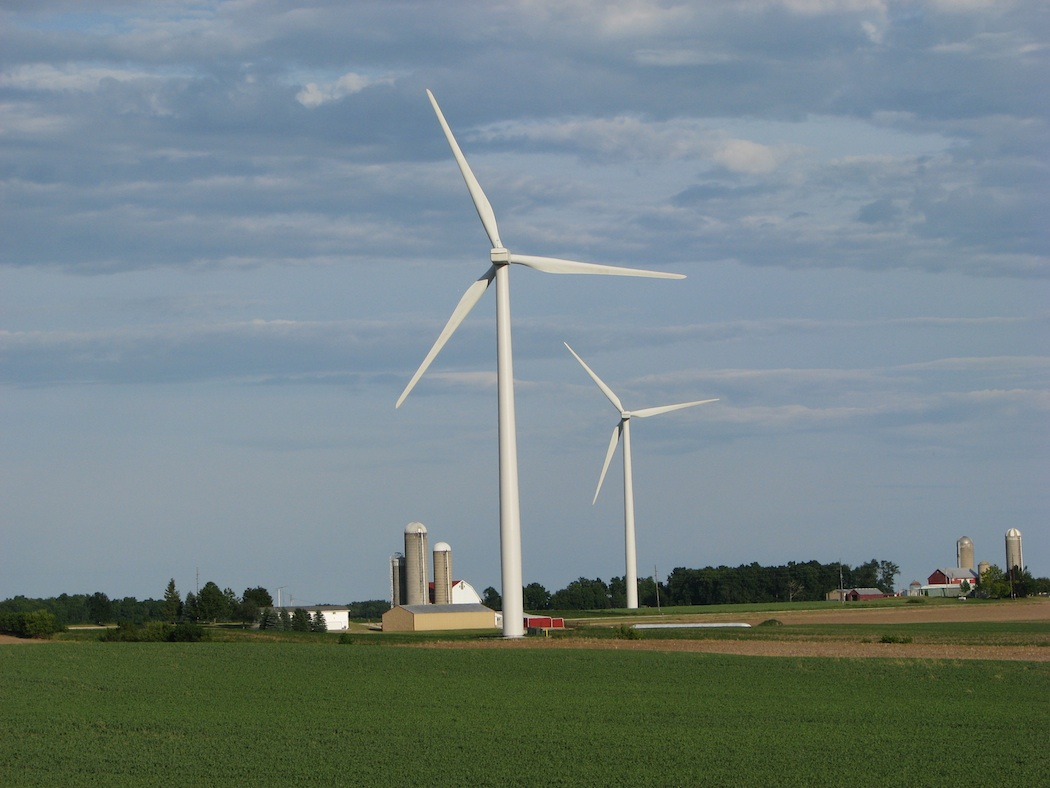
\includegraphics[height=2.5in]{files/21206}}
\hfill 
\subfigure[Aerial view of the National Wind Technology Center. 
 (Photo by Dennis Schroeder / NREL)\label{fig:20018}]
 {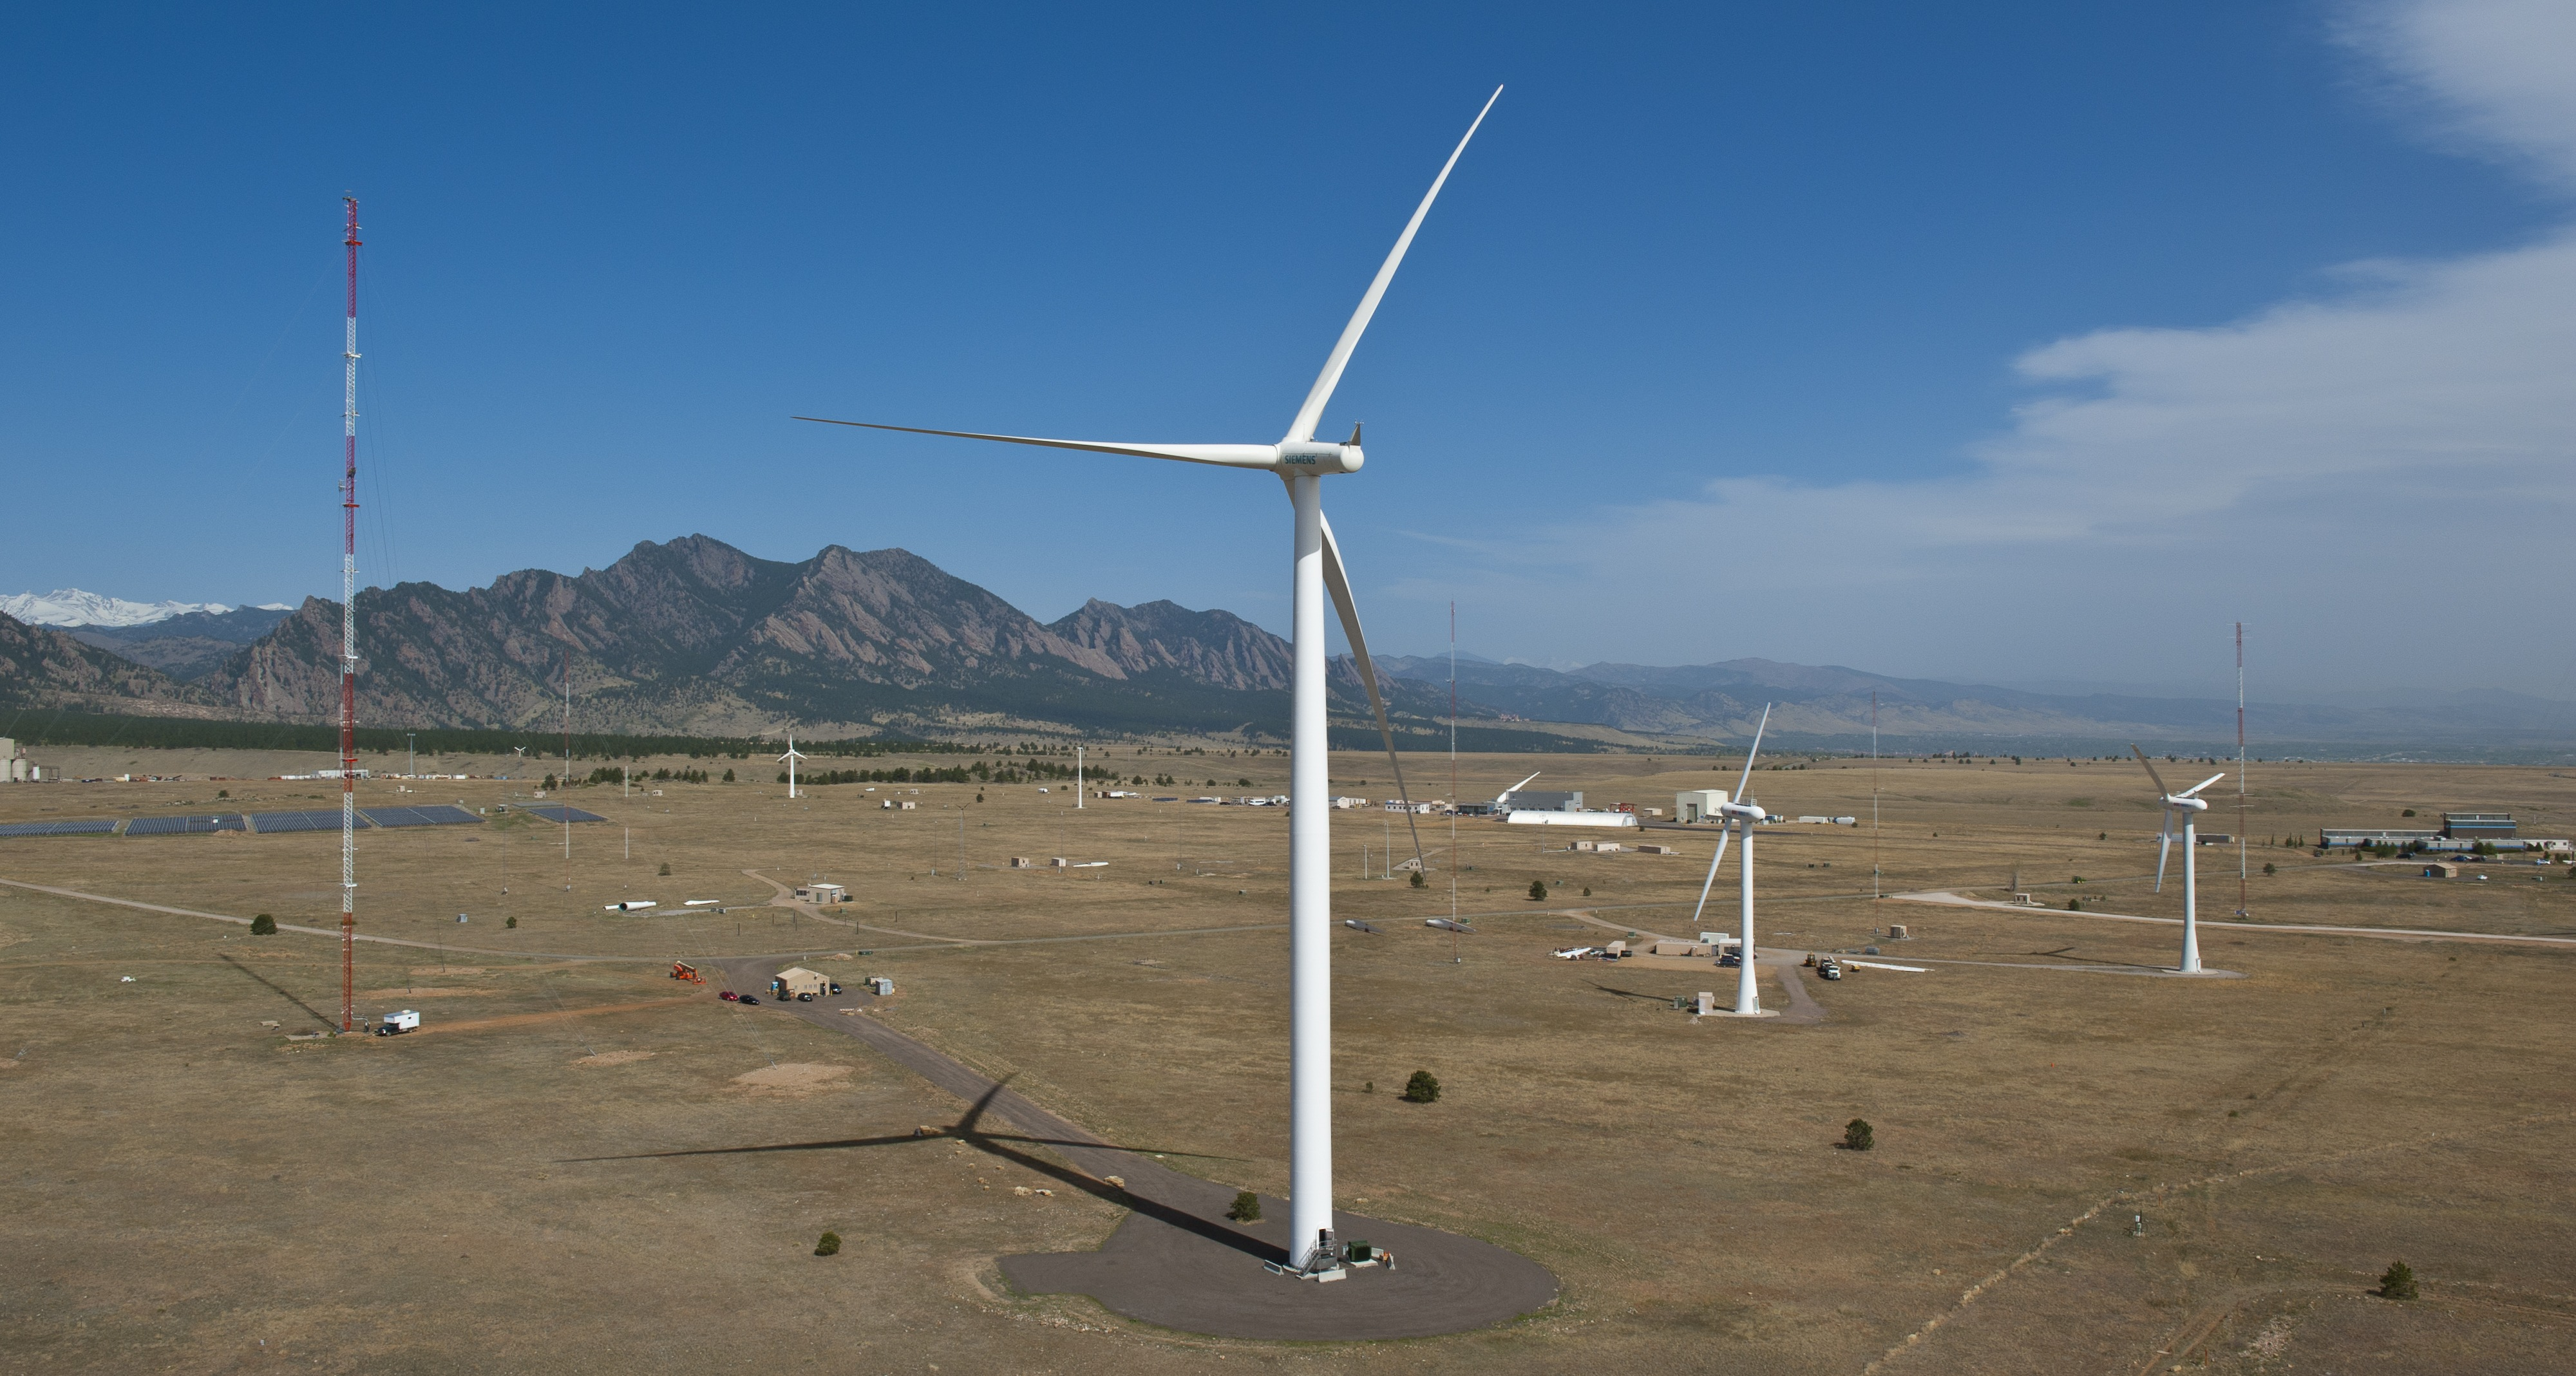
\includegraphics[height=2.5in]{files/20018}}
\hfill
\caption{NREL images}\label{fig:NRELimages}
\end{figure}
\end{verbatim}
 
\begin{figure*}[htp]
\centering
\hfill
\subfigure[Wind turbines at the Forward Wind Energy Center in Fond du Lac and Dodge Counties, Wisconsin. (Photo by Ruth Baranowski / NREL)\label{fig:21206}]{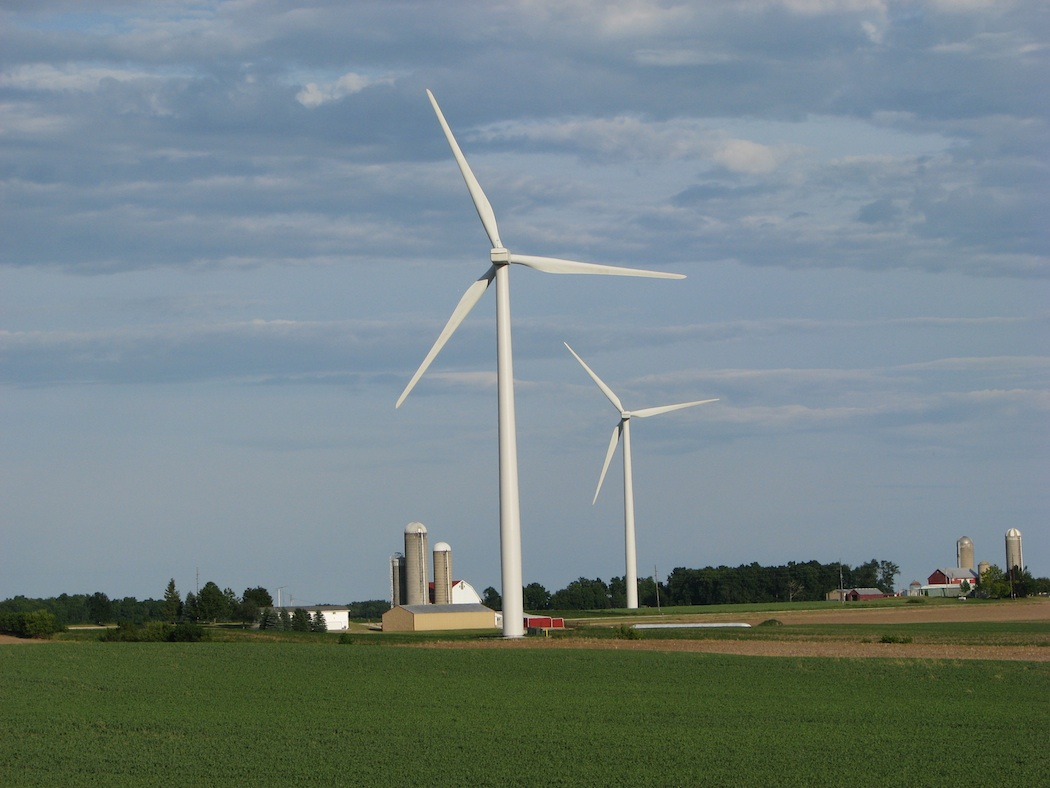
\includegraphics[height=2.5in]{files/21206}}
~ %add desired spacing between images, e. g. ~, \quad, \qquad etc. (or a blank line to force the subfigure onto a new line)
\hfill
\subfigure[Aerial view of the National Wind Technology Center. (Photo by Dennis Schroeder / NREL)\label{fig:20018}]{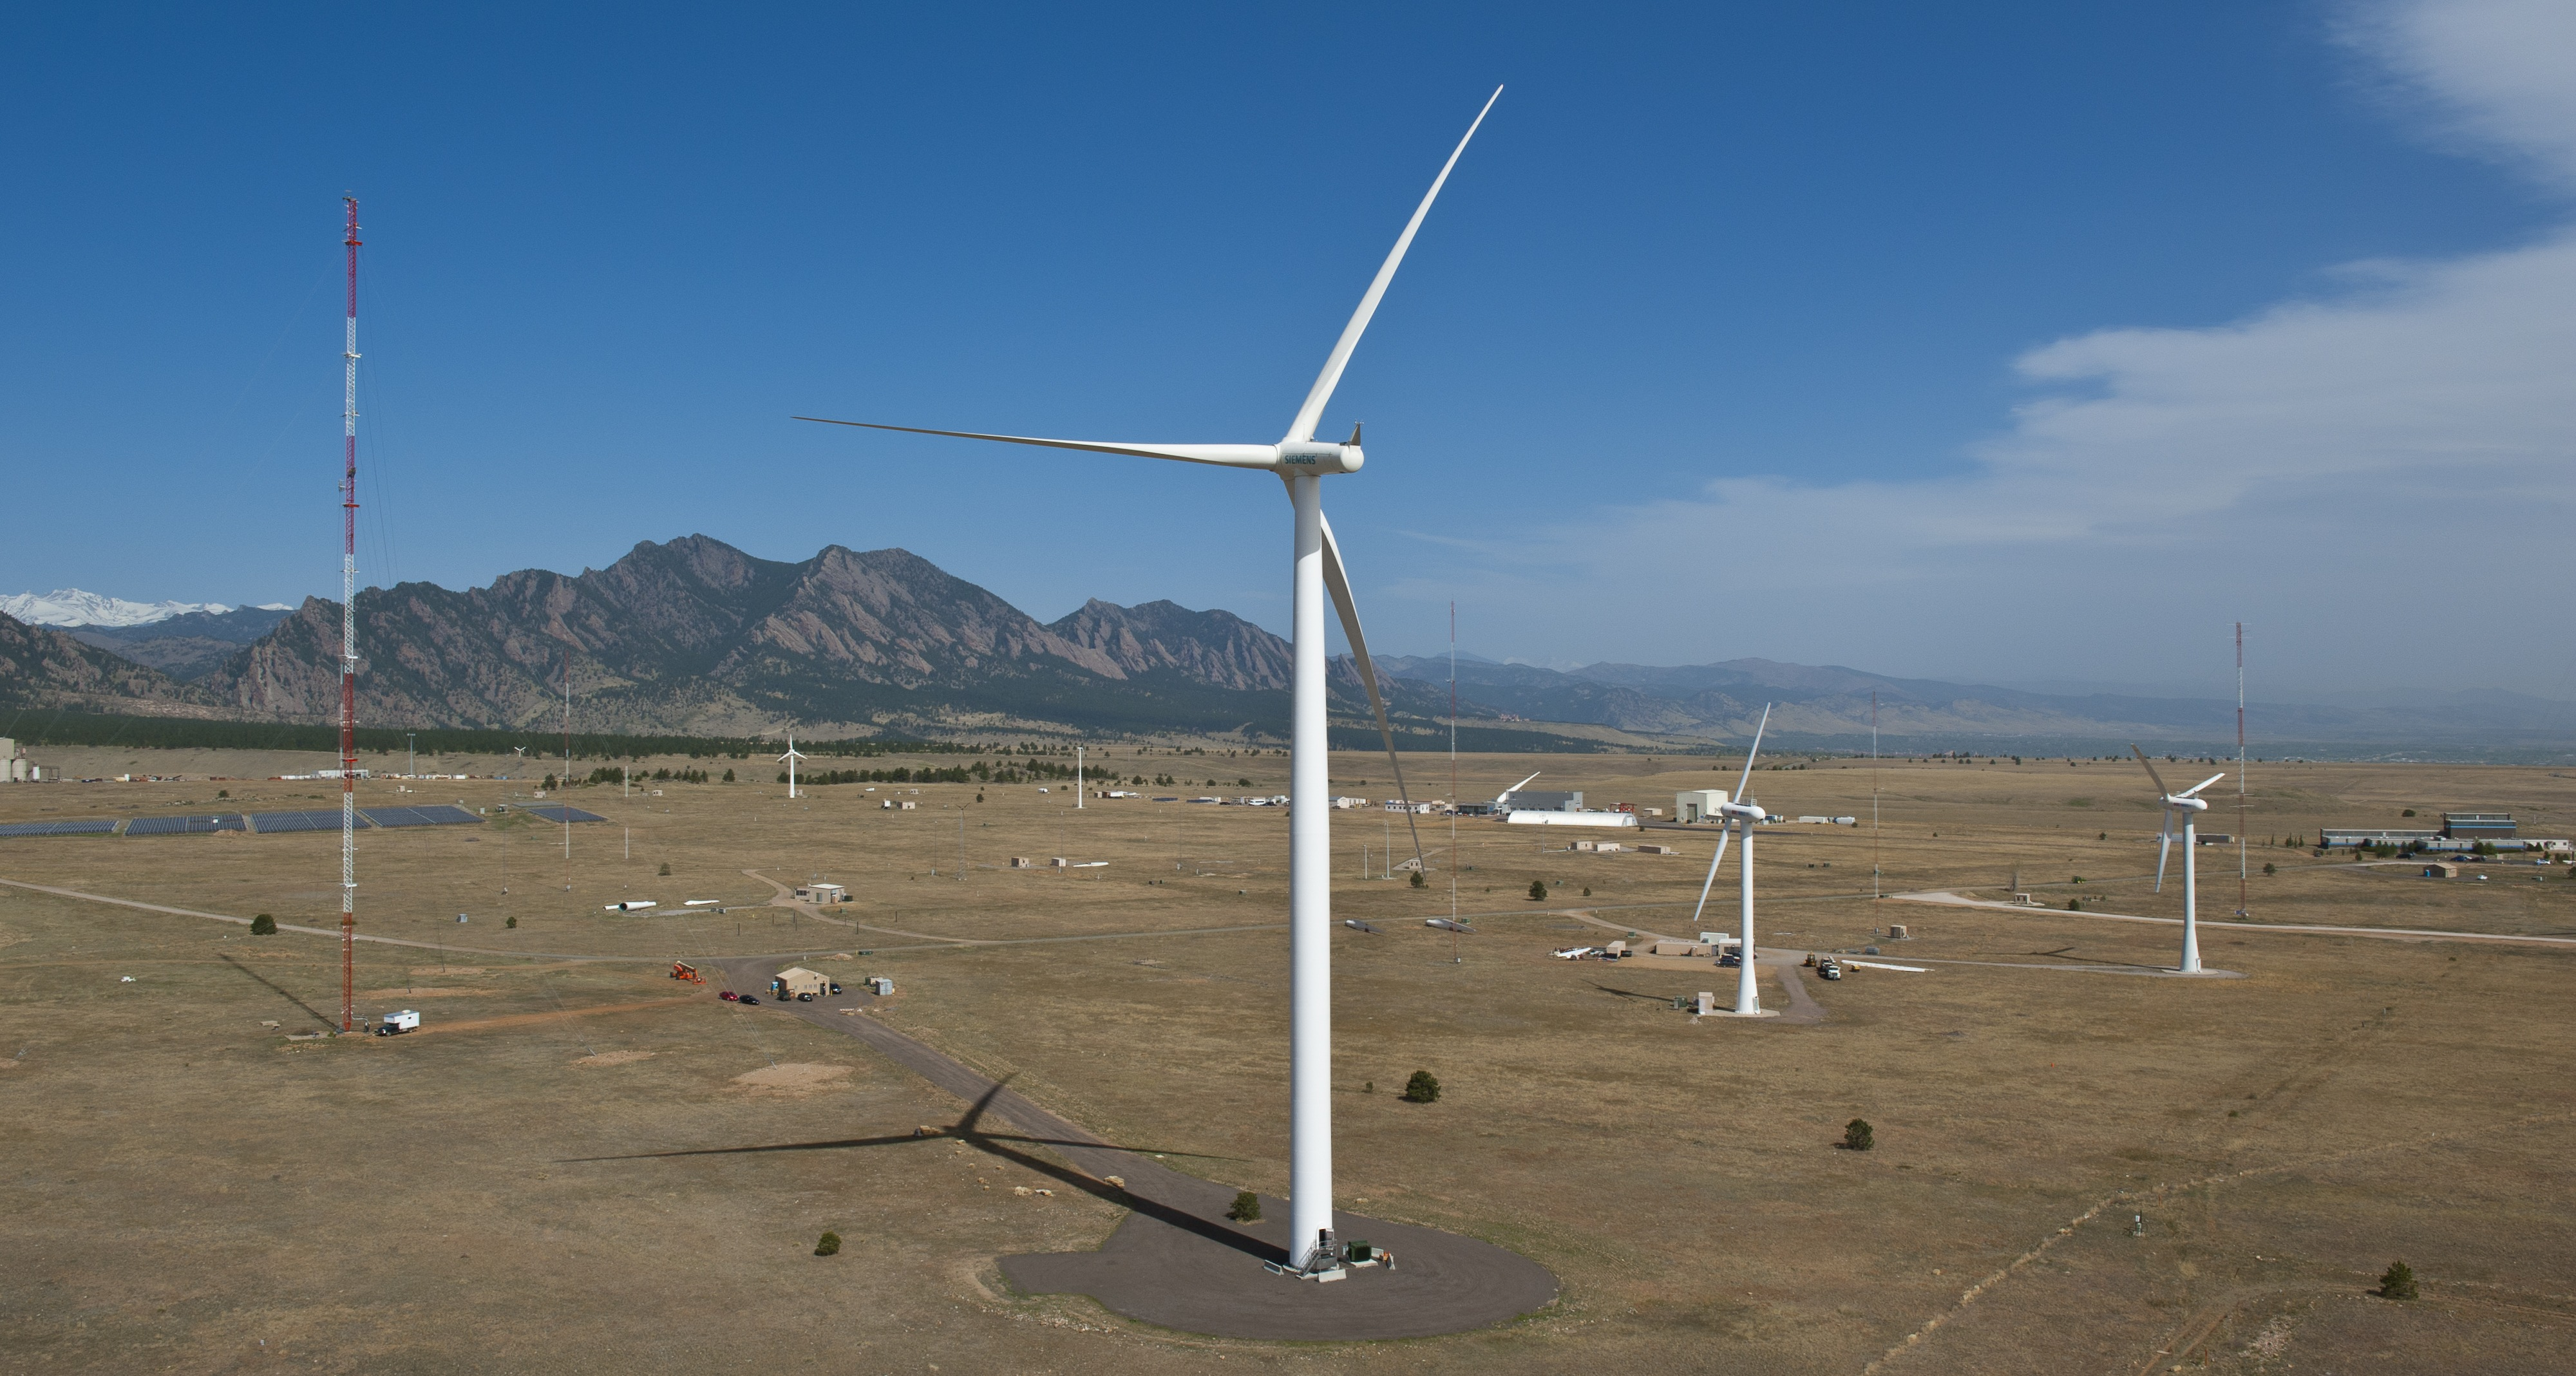
\includegraphics[height=2.5in]{files/20018}}
\hfill
\caption{NREL images}\label{fig:NRELimages}
\end{figure*}

If a subfigure is split over two lines using \verb+\\+, make sure those symbols are on their own line.

\section{Citations}
\label{Sec:Bib}
Use \texttt{bibtex} to organize references and store them in a single file (e.g. \verb+/Documents/bibliography/bibliography.bib+). The bibliography will then contain entries with `keys', like \texttt{Lamport\_1986\_a}. Authors can then insert citations to this key throughout their document, using different styles of citation. These are describe in the \emph{achicago.sty} documentation.
\begin{itemize}
\item \verb+\cite{Lamport_1986_a}+ prints \cite{Lamport_1986_a}.
\item \verb+\citep{Lamport_1986_a}+ prints \citep{Lamport_1986_a}.
\item \verb+\citet{Lamport_1986_a}+ prints \citet{Lamport_1986_a}.
\end{itemize}

To cite URLs, use the 'misc' style. For example, the bibtex entry for \href{http://tex.stackexchange.com}{http://tex.stackexchange.com}\ \cite{texstackexchange} looks like this:

\begin{verbatim}
@misc{texstackexchange,
	Author = {Anon.},
	Howpublished = {Accessed July 21, 2014: \url{http://tex.stackexchange.com}},
	Title = {\TeX -- LaTeX Stack Exchange},
	Year = {2014}}
\end{verbatim}

This format will allow you to include the date on which a URL was accessed.

The citations should work with journal articles, books \citep{Lamport_1986_a}, technical reports \citep{TechReportTest}, and URLs \citep{texstackexchange}.

\section{Computer code}
The \texttt{lstlisting} package has been loaded.

\section{NREL-style bibliographies}
NREL uses "Chicago A" style-references. The \emph{nrel.cls} file uses Biblatex to produce these references. To include a bibliography in the document, use the following commands where you want the bibliography to occur:

\begin{verbatim}
\bibliography{files/bibliography.bib}
...
\begin{document}
...
\cleardoublepage
\label{sec:Bib}
\printbibliography
...
\end{document}
\end{verbatim}

\section{Creating a file structure}
\label{sec:FileStructure}
Use the \texttt{input} command to import other files into your main file. For example, each of the chapters in this report could be in separate files, called \emph{NRELRequirements.tex} (Chapter 1), \emph{LatexAtNREL.tex} (Chapter 2), and so-on. 

\begin{verbatim}
...
\begin{document}
% content
\input{NRELRequirements}
\input{LatexAtNREL}
\input{ConvertingToDoc}
...
\end{verbatim}

\section{Putting it all together}
The source of your LaTeX document should probably look like this:

\begin{verbatim}
\newif\iflatextortf
\iflatextortf
 % tell latex2tortf if this is an article or report
 \documentclass[10pt,letterpaper]{report}
 % File NRELLatex2rtf.tex

% set margins
\usepackage[margin=1 in,letterpaper]{geometry}

% use citations
\usepackage[sort]{natbib}

% change the heading of the bibliography
\renewcommand{\bibsection}{\section{References}}

% redefine \pdftooltip so that it behaves differently with and without latextortf
\newcommand{\pdftooltip}[3][]{#2}

%redefine the checkmark
\newcommand{\checkmark}{y\relax}

% redefine booktabs commands
\newcommand{\toprule}{\hline}
\newcommand{\midrule}{\hline}
\newcommand{\bottomrule}{\hline}

% redefine \href
\newcommand{\href}[2]{#1~ (\url{#2})}

% redefine \subfloat to match the \subfigure environment
\usepackage{subfigure}
\makeatletter
\newcommand{\subfloat}[2][]{\subfigure{\textit{Subcaption: \protect{#1}}}{#2}}
%\newcommand{\subfloat}[3][]{\subfigure{#1}{#2}{#3}}
% note that we can only have one '\label' in a figure environment
\makeatother

\newcommand{\subref}[1][]{\ref{#1}}

% redefine \todo so that it gives something useful
\newcommand{\todo}[2][]{\textbf{To Do:}~#2}

% deal with index entries:
\newcommand{\index}[1]{}
\else
 \documentclass[draft,report]{nrel} 
\fi
\title{Writing NREL documents using LaTeX}
\author{A. Clifton, A. Platt, P. Fleming, M. Lawson}
\bibliography{files/bibliography.bib}
\begin{document}
\maketitle
\frontmatter
\input{ExecSummary}
\tableofcontents
\clearpage
\listoffigures
\listoftables
\mainmatter
\input{Introduction}
\input{Theory}
\cleardoublepage
\label{sec:Bib}
\printbibliography

\end{document}
\end{verbatim}

\section{Best practice in writing a document in LaTeX}
\begin{description}
\item[Create a structure before you get too far.] Authors will find it easier to write documents and make changes if they separate the content of the document from the structure.
\begin{enumerate}
\item Each new LaTeX document should be placed in it's own directory. 
\item Create a main LaTeX file that just contains the preamble, custom commands and uses \texttt{input} to call the content. See Section \ref{sec:FileStructure} for an example where each \texttt{chapter} is contained in its own file. In an article, each \texttt{section} could be contained in its own file.
\item Keep the number of packages used to a minimum. If authors feel that something is desperately missing, they can contact the maintainers of the \emph{nrel.cls} file. Not all packages can be used as they lack compatibility.
\end{enumerate}
\item[Focus on content, not appearance.] Don't spend hours trying to adjust fonts, headers or spacing between lines. 
\begin{enumerate}
\item The document produced should meet NREL's requirements if it is compiled using \emph{nrel.cls}. 
\item Don't throw in lots of \texttt{clearpage}s or other commands to push material around. LaTeX is designed to handle that. 
\item Resist the temptation to add or subtract space, change lengths or do other things to modify the layout. 
\item Write!
\end{enumerate}
\end{description}
